\chapter{RNA Motifs}
\label{motifs} 
\bibliographystyle{nar}

\section{RNA \textit{Structural} Motifs}
The following popular definitions of what an ``\textit{RNA structural
  motifs}'' is, can be found in recent literature:
\begin{itemize}
\item{RNA motifs are ``\textit{Conserved  structural subunits that  make up the  secondary
structures of RNAs.}''\cite{holbrook2005}}
\item{RNA motifs are ``\textit{Ordered stacked arrays of
non-Watson-Crick  base pairs that  form distinct  folds  on  the
phosphodiester backbones of  RNA strands.}''\cite{leontis2003}} 
\item{``\textit{An RNA Motif is a discrete sequence or combination of base
juxtapositions found in naturally occurring RNA's in unexpectedly high
abundance.}''\cite{moore1999}}
\end{itemize}
First, a word of caution must be given to the reader. The term
``\textit{RNA motif}'' alone, can be used to describe three different
levels of RNA organization, that is, RNA sequence motifs, RNA
secondary structure motifs, or RNA 3D structure motifs. We start by
making such distinction as it is not always clearly mentioned in RNA
literature, generating a great deal of confusion and bibliographical
search frustration for the beginner. In the remaining of
this text it is to be understood that RNA structural motifs refer to
specific geometrical arrangements in three dimensional space.

As can be seen from the previous definitions, and from the introduction, 
there is no unique,
or consensus definition of what an RNA structural motif is yet, and it
seems like every researcher has it's own, even if they don't declare
them. The RNA Ontology Consortium (ROC) has not come to a consensus
definition or RNA structural motifs neither. The majority of their
work has been centered at understanding RNA backbone conformations, and
the influence of isosteric substitutions on RNA structure. The
ROC has yet to address the relation of base-staking to RNA structural
motifs, which leaves a natural space for the rigid-block interpretation
of nucleic acids to fill in.

\section{GNRA tetraloop}
In order to compare our work to that of others on RNA structural motif
localization and discovery, we ask the following questions:
\begin{enumerate}
\item{Can the geometric rigid-block description of base-pairing and
base-stacking solve the problem of defining RNA structural motifs?}
\item{Can we use quantities derived from the 3DNA software package to make
and automatic search for a known motif, for example, the GNRA
tetraloop motif, and perhaps find unknown motifs?}
\end{enumerate}
In the ROC meeting of May, 2009 a reduced dataset of RNA
structures found at:\\
http://docs.google.com/Doc?id=dhrmkfmn\_13ftpbjcgq\\
was made available to participants with the purpose of allowing
them to search for RNA motifs, which would later be compared between groups.

We have modestly, and as of yet unsuccessfully, started to aim at solving
question number two. Initially we are trying to identify all
instances of the well known GNRA tetraloop motif in
the 23S subunit of ribosomal RNA of \textit{Thermus Thermophilus},
PDB-ID:1ffk using results from 3DNA and 3DNA-Parser, and using an
automated process which could be later reproduced for any desired dataset.
Our hope is that these baby steps will allow us to to tackle the whole ROC dataset.

\subsection{3DNA-Parser}
We started by using Dr. Yurong Xin's 3DNA-Parser hoping that the
description of the enclosing base pair in the loop, that is, the
sheared G$\cdot$A, would have a characteristic signature.
We found that such is not the case. We know from Major et
al. \cite{lemieux2006} that there should be at least 21 GNRA tetraloops
in the 23S subunit of rRNA. We used the G2696 N2697 R2698 A2699
tetraloop as a seed (as can be seen in Figure 1.1) and found out
that according to Dr. Xin's helical classification the enclosing G is
classified as $S_{hq}$ and A is classified as $H_{e}$. 
\begin{figure}[htbp]
\centering 
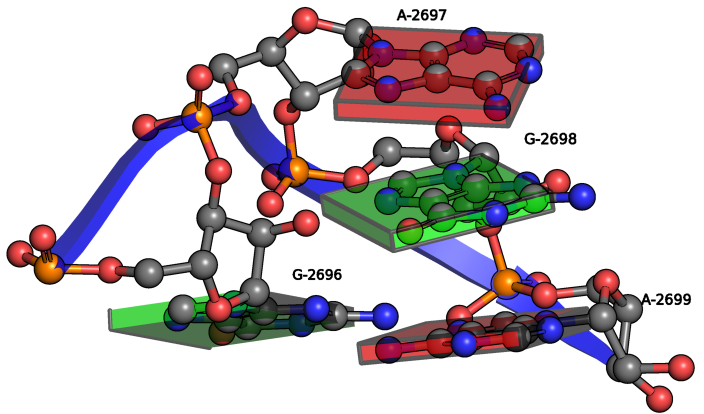
\includegraphics[angle=0, scale=0.5]{Chapter5/gnra.png}
\caption{GNRA Tetraloop from \textit{Thermus Thermophilus} 23S Ribosomal RNA PDB-ID:1ffk.}
\end{figure}
We then searched all such instances for G$\cdot$A base-pairs and we found seven hits,
but none were in fact GNRA tetraloops.

\subsection{Overlap Scores} 
We also used 3DNA overlap scores hoping to assign RNA structural motifs to
evident patterns formed after data clustering.
We tried out a sliding sequence window, meaning that we make a
vector whose components are the overlap values shifted by one
base, for example, if we had the sequence GAUAGAC, they will
correspond to the following sequences:\\
\\
GAUA\\
AUAG\\
UAGA\\
AGAC\\

Each being represented by a three dimensional vector whose components
are the overlaps between consecutive bases.
The results after clustering are shown in Figure 1.2.,  from which it's clear that
there are no obvious groups being ``formed".
\begin{figure}[htbp]
\centering 
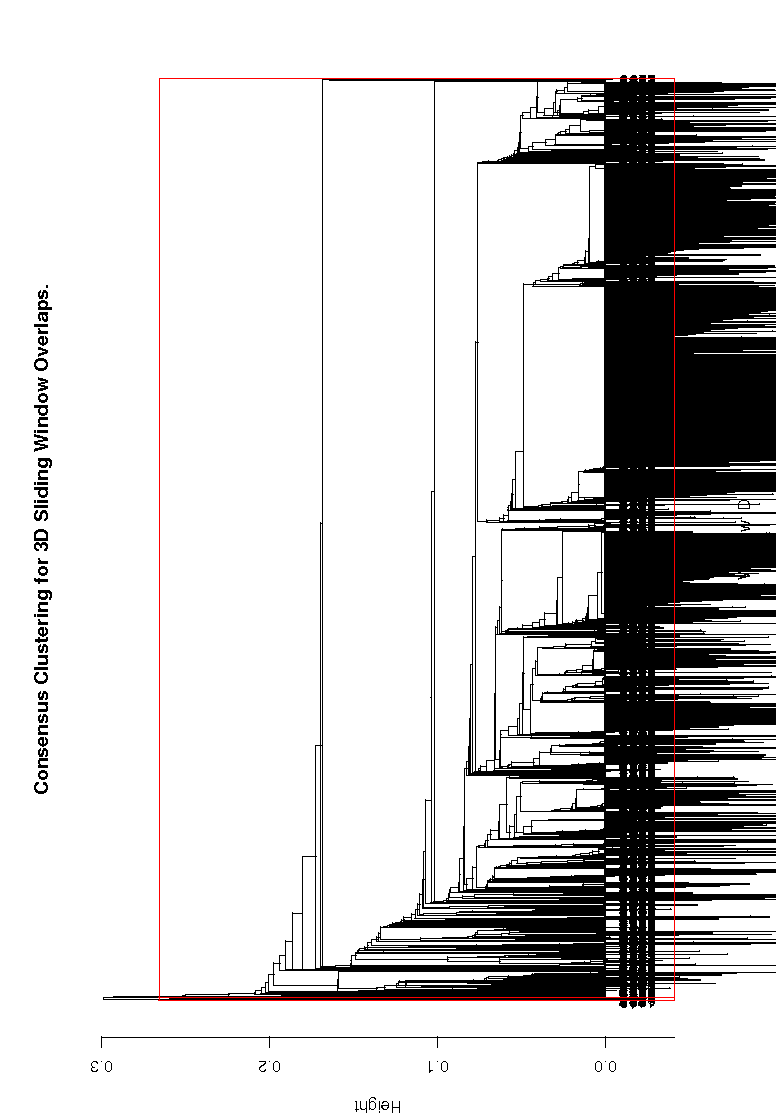
\includegraphics[angle=0, scale=0.8]{Chapter5/3Dwindow.png}
\caption{Dendrogram for consensus clustering of 3D sequential
overlaps. All vector elements were normalized.}
\end{figure}
Perhaps we should increase the size of
the sliding window, at least to five bases, and include residue identity as
an additional dimension.

We also clustered the overlap values in one dimension and got rid of
all overlap values which were zero. One reason for justifying this approach 
is that there are so many values which are exactly zero (33\%), that all other data
is overshadowed (This can be seen clearly for the normalized histograms in Figure).
\begin{figure}[htbp]
\centering 
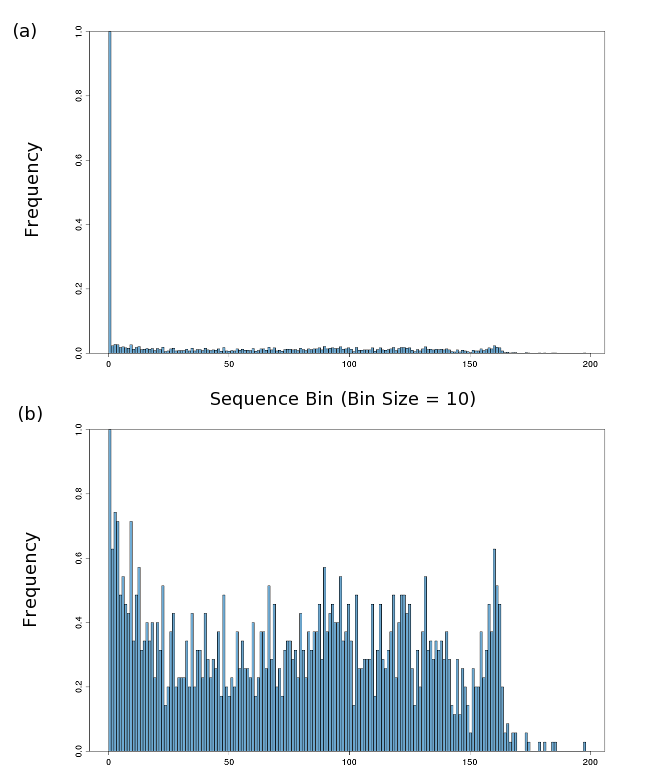
\includegraphics[angle=0, scale=0.8]{Chapter5/histocompare.png}
\caption{Normalized histograms showing the distribution of overlap values in 
the 23S subunit or \textit{Thermus Thermophilus} rRNA, PDB-ID:1jjk. In histogram 
(a) all values are included, but in histogram (b) only values greater than zero are 
included. Notice the high preponderance of zero values, exactly 897 out of a total
of 2705.}
\end{figure}
For this case we obtained a ``good'' dendrogram as seen in Figure 1.3, but the interpretation is
difficult since it's only good for continuously stacked regions, therefore not
general, and it might be introducing an unwanted artifact.
\begin{figure}[htbp]
\centering 
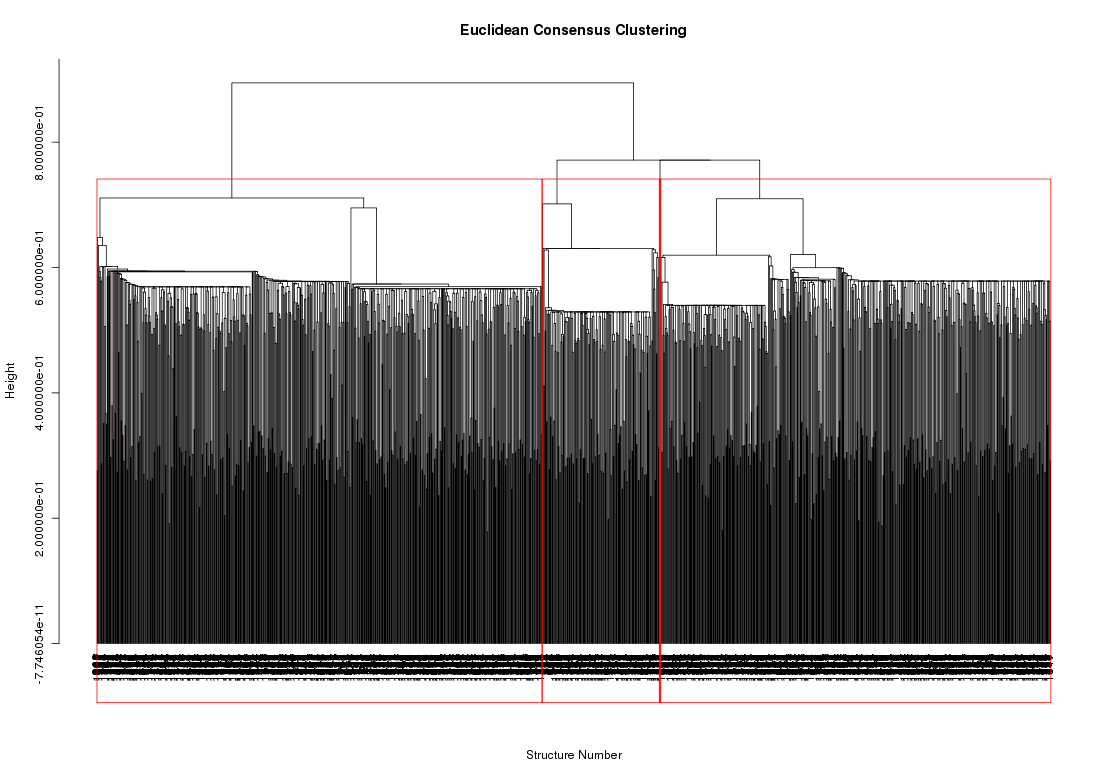
\includegraphics[angle=90, scale=0.6]{Chapter5/eucli_cons.png}
\caption{Dendrogram for consensus clustering of 1D sequential overlaps
  with zero values filtered out and vector elements normalized to unity.}
\end{figure}
The next step in this analysis will be to find the structures which
correspond to this clusters and superimpose and align them using
Kabsh's algorithm to be able to determine their RMSD's.

Many people start their RNA Motif identification and classification
algorithms by splitting RNA structures into what is helical and what
is not, and then finding interactions between these two groups. We
believe that we could do a similar exercise with 3DNA by using the scalar
product of helical axis vectors and once helical and non-helical
regions are found we might be able to use 3DNA Parser to look for characteristic
interactions.

\section{Triplets on RNA (comparison to Laing et al.)}


\bibliography{biblio}

